\chapter{Utilizzo di un opamp}

\section*{Obiettivo}

Testare i vari amplificatori operazionali e analizzare la loro risposta in frequenza.
\section*{Svolgimento}
\subsection*{OP37\footnote{\href{https://www.analog.com/media/en/technical-documentation/data-sheets/OP37.pdf}{Datasheet OP37}}}
%%TODO aggiungere cose vecchie
L'opamp OP37 è stabile con un guadagno >= 5. 
Proviamo ad impostare, usando l'opamp in configuarazione non invertente, un guadagno inferiore per vedere come si comporta.

\begin{figure}[H]
\centering
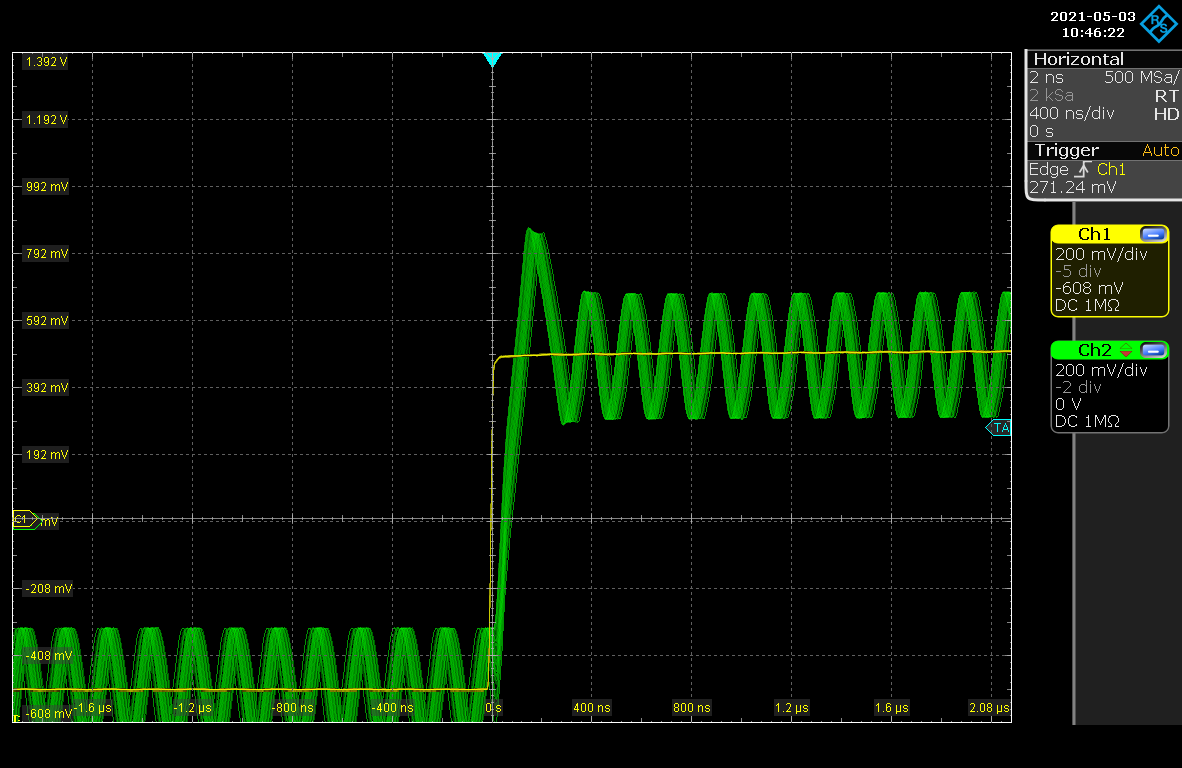
\includegraphics[width=\textwidth]{assets/exp8/Guadagno_1.png}
\caption{Guadagno 1}
\end{figure}

\begin{figure}[H]
\centering
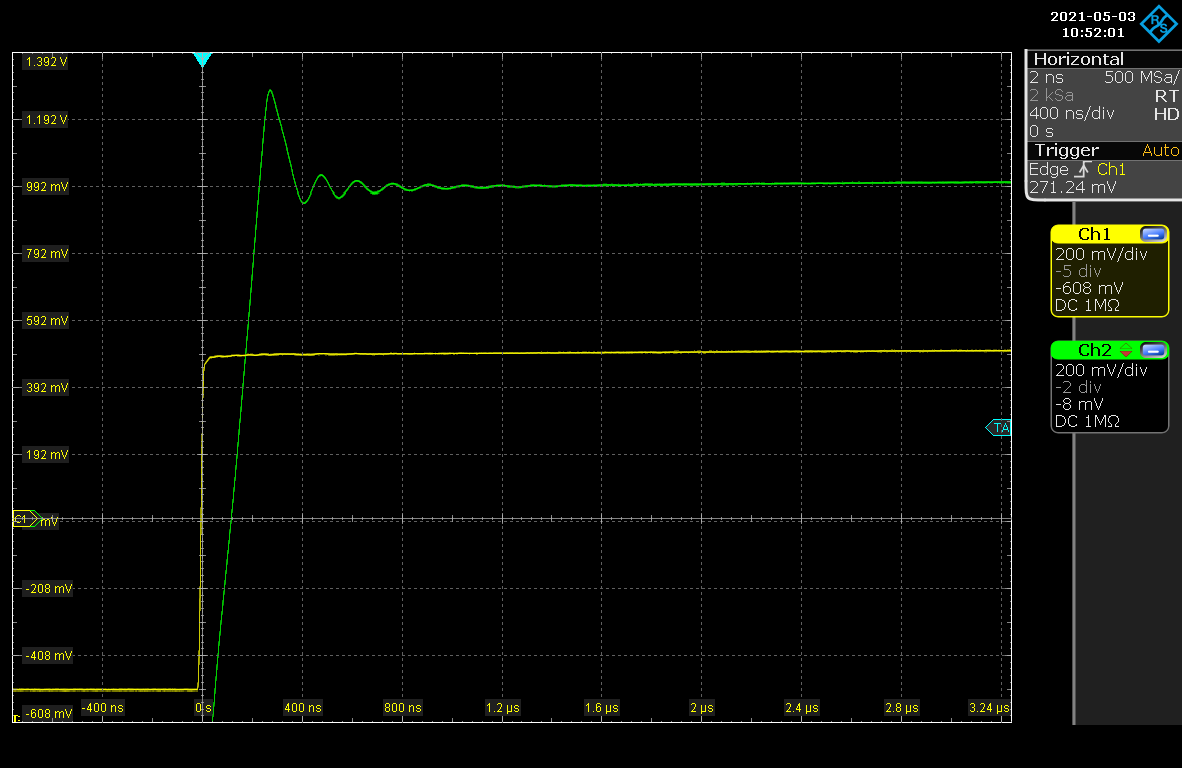
\includegraphics[width=\textwidth]{assets/exp8/Guadagno_2.png}
\caption{Guadagno 2}
\end{figure}

Impostando invece un guadagno superiore a 5 notiamo un comportamento stabile dell'amplificatore.
\begin{figure}[H]
\centering
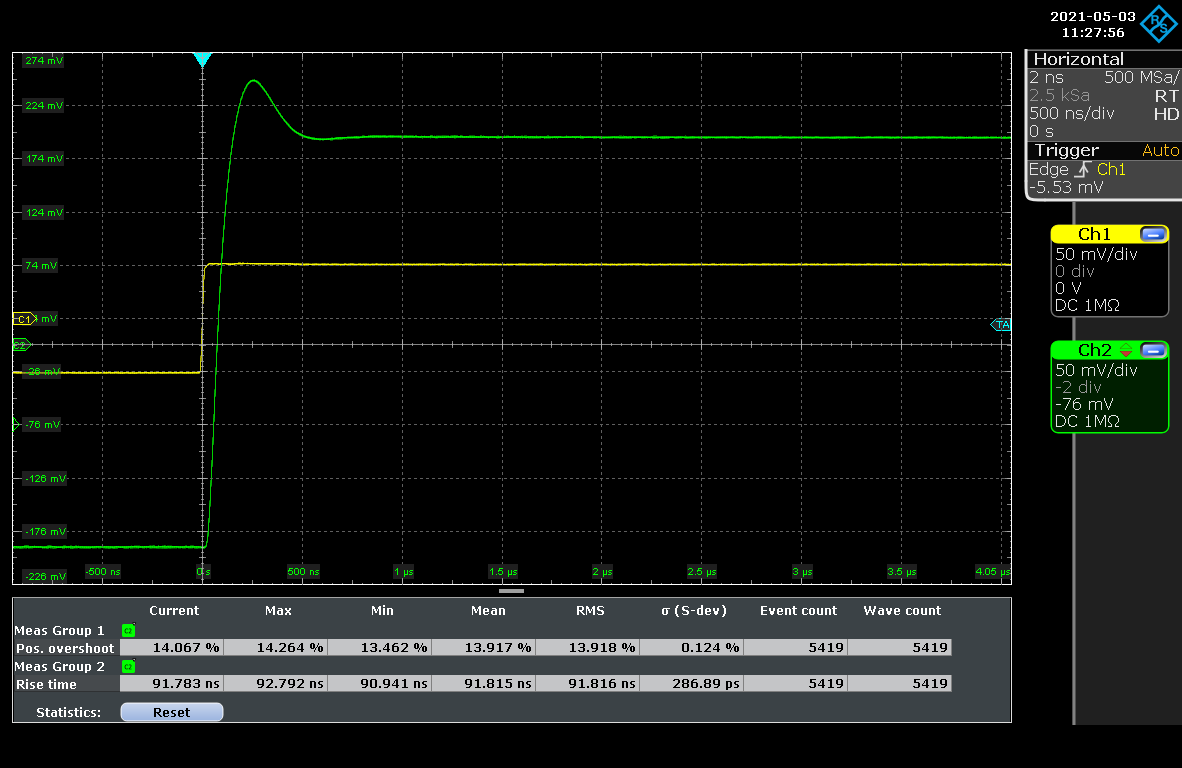
\includegraphics[width=\textwidth]{assets/exp8/Guadagno_7.6666_pt2.png}
\caption{Guadagno 7.6}
\end{figure}

Proviamo anche l'opamp in configurazione invertente.
\begin{figure}[H]
\centering
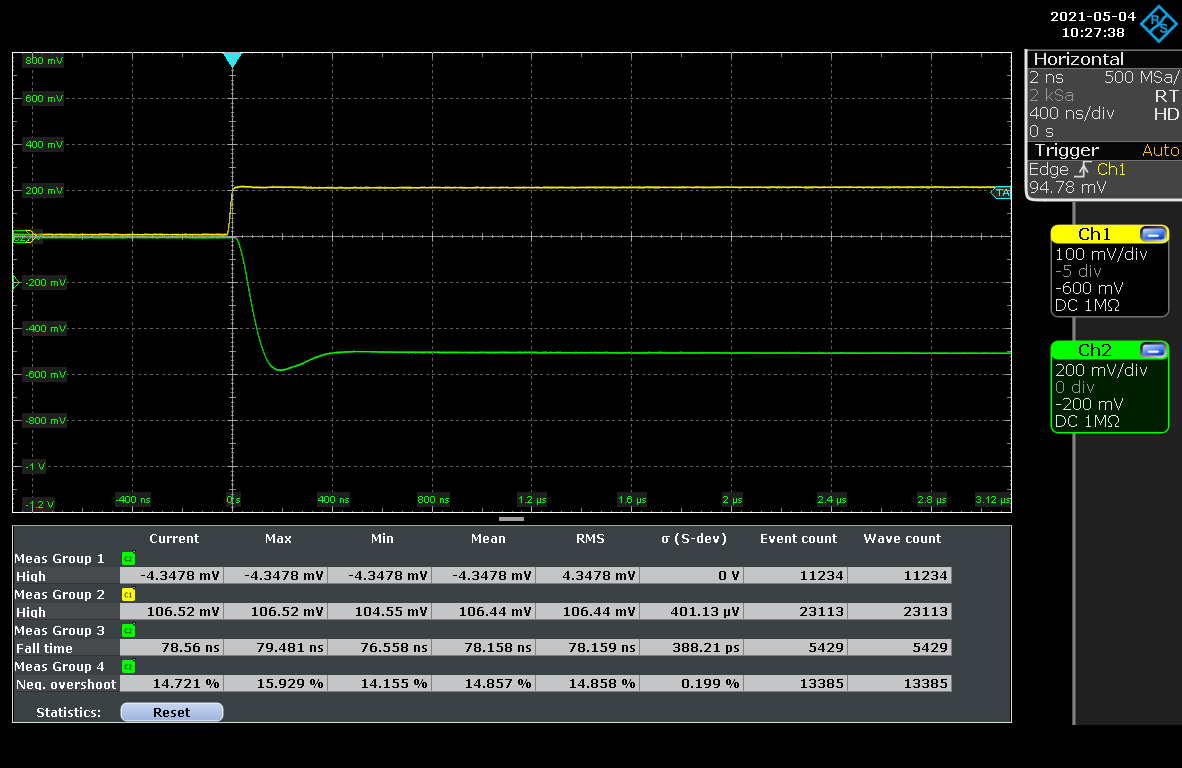
\includegraphics[width=\textwidth]{assets/exp8/invertente.png}
\caption{Configurazione invertente}
\end{figure}

Proviamo ad impostare con il generatore di funzioni una sinusoide con frequenza via via maggiore (da 1MHz a 10Hz) e vediamo come il guadagno dell'opamp vada a diminuire con l'aumentare della frequenza.

\begin{figure}[H]
\centering
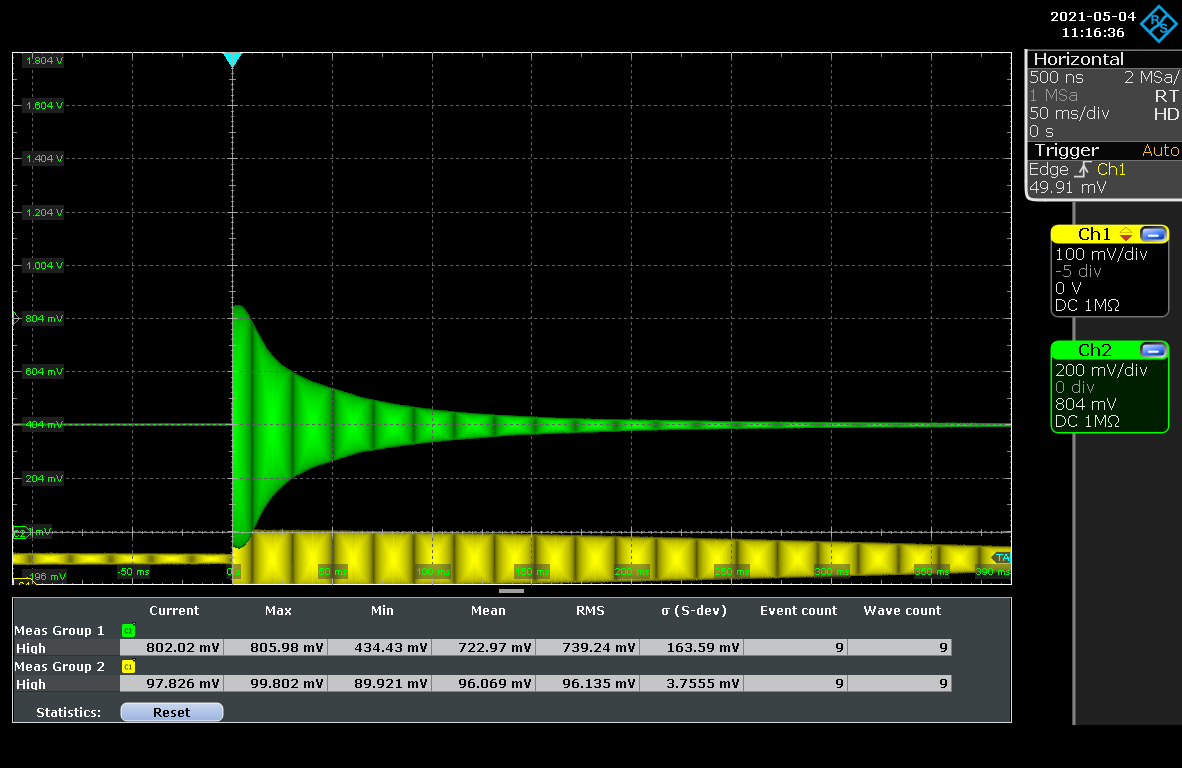
\includegraphics[width=\textwidth]{assets/exp8/Screenshot_2021-05-04_1_111636.png}
\caption{Configurazione invertente}
\end{figure}



\subsection*{AD9631\footnote{\href{https://www.analog.com/media/en/technical-documentation/data-sheets/AD9631_9632.pdf}{Datasheet AD9631}}}

Misuriamo il tempo di rise dell'opamp AD9631 prendendo in considerazione anche il tempo di rise del generatore di funzioni.

Sappiamo che il tempo di rise al netto del tempo di rise del generatore di funzioni è dato dalla seguente formula:

\begin{displaymath}
 \sqrt{tRiseOpAmp^2 - tRiseFunctGen^2}
\end{displaymath}

Quindi nel nostro caso il tempo di rise è 40.29 nsecondi.

\begin{figure}[H]
\centering
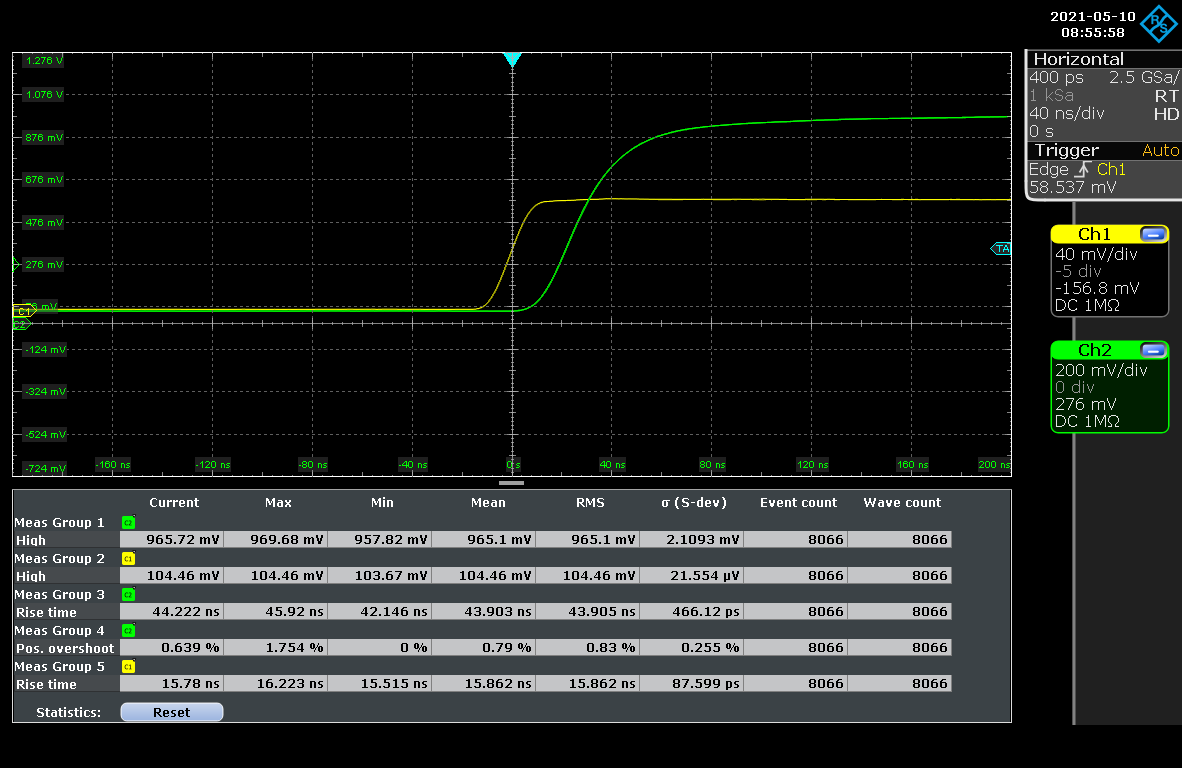
\includegraphics[width=\textwidth]{assets/exp8/Screenshot_2021-05-10_0_085558.png}
\end{figure}

Condizioni dell'esperimento:
\begin{itemize}
    \item OPAMP AD9631
    \begin{itemize}
        \item R1: 910 ohm
        \item R2: 110 ohm
        \item Gain: 9.27
    \end{itemize}
    
    \item Funzione generata:
    \begin{itemize}
        \item Onda quadra a 1khz
        \item Amplitude: 102mV
        \item High: 103mV
    \end{itemize}
    
\end{itemize}


%% cose particelle

primo stadio già fatto dai prof. converte corrente in tensione
mettere immagine solo giallo

Mettiamo il secondo opamp in configurazione invertente.
RF = 110 ohm
R1 = 22 ohm 
guadagno = 5

immagine giallo + verde

Proviamo con gain 50 
RF = 11000
R1 = 2000


freq impulsi
4 in 50 microsec
FARE COSE CON ACQUSITION

ISTOGRAMMA

